\documentclass[11pt]{article}
\usepackage{amsmath,amsthm,stmaryrd,amsfonts}
\usepackage{tikz}
\usetikzlibrary{shapes.geometric, arrows}

\begin{document}

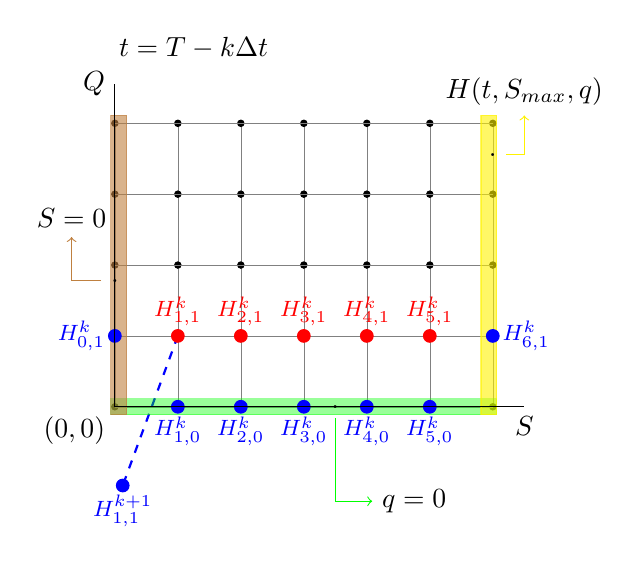
\begin{tikzpicture}
	\foreach \x in {-2.4,-1.6,-0.8,...,3.2}
	{
		\draw[very thin, gray] (\x,-1.8) -- (\x,1.8);
		\foreach \y in {-1.8,-0.9,...,2.7}
		{
			\filldraw (\x,\y) circle (0.04);
		}
	}
	\foreach \y in {-1.8,-0.9,...,2.7}
	{
		\draw[very thin, gray] (-2.4,\y) -- (2.4,\y);
	}
	\draw (-2.4,-1.8) node[below left] {$(0,0)$};
	\draw[blue,thick,dashed] (-1.6,-0.9) - - (-2.3,-2.8);
	\filldraw[blue](-2.3,-2.8) circle (0.08) node[below] {\footnotesize $H_{1,1}^{k+1}$};	
	\filldraw[color=green,opacity=0.4] (-2.45,-1.9) -- (2.45,-1.9) -- (2.45,-1.7) -- (-2.45,-1.7) --cycle;
	\filldraw[color=brown,opacity=0.6] (-2.45,-1.9) -- (-2.45,1.9) -- (-2.25,1.9) -- (-2.25,-1.9) --cycle;
	\filldraw[color=yellow,opacity=0.6] (2.45,-1.9) -- (2.45,1.9) -- (2.25,1.9) -- (2.25,-1.9) --cycle;	
	\filldraw[blue](-1.6,-1.8) circle (0.08) node[below] {\footnotesize $H_{1,0}^k$};
	\filldraw[blue](-0.8,-1.8) circle (0.08) node[below] {\footnotesize $H_{2,0}^k$};
	\filldraw[blue](0.0,-1.8) circle (0.08) node[below] {\footnotesize $H_{3,0}^k$};
	\filldraw[blue](0.8,-1.8) circle (0.08) node[below] {\footnotesize $H_{4,0}^k$};
	\filldraw[blue](1.6,-1.8) circle (0.08) node[below] {\footnotesize $H_{5,0}^k$};
	\filldraw[blue](-2.4,-0.9) circle (0.08) node[left] {\footnotesize $H_{0,1}^k$};
	\filldraw[red](-1.6,-0.9) circle (0.08) node[above] {\footnotesize $H_{1,1}^k$};
	\filldraw[red](-0.8,-0.9) circle (0.08) node[above] {\footnotesize $H_{2,1}^k$};
	\filldraw[red](0.0,-0.9) circle (0.08) node[above] {\footnotesize $H_{3,1}^k$};
	\filldraw[red](0.8,-0.9) circle (0.08) node[above] {\footnotesize $H_{4,1}^k$};
	\filldraw[red](1.6,-0.9) circle (0.08) node[above] {\footnotesize $H_{5,1}^k$};	
	\filldraw[blue](2.4,-0.9) circle (0.08) node[right] {\footnotesize $H_{6,1}^k$};
	%nodes
	\node (A) at (-2.4,-0.2){.};
	\node (B) at (-2.95, 0.6) {$S=0$};
	\node (C) at (0.4,-1.8) {.};
	\node (D) at (1.4, -3.0) {$q=0$};
	\node (E) at (2.4,1.4) {.};
	\node (F) at (2.8,2.2) {$H(t,S_{max},q)$};
	% arrows
	\draw[brown][->, to path={-| (\tikztotarget)}]
	(A) edge (B);
	\draw[yellow][->, to path={-| (\tikztotarget)}]
	(E) edge (F);
	\draw[green][->, to path={|- (\tikztotarget)}]
	(C) edge (D);
	
	\draw[black] (-1.4, 2.5) node[above] {$t=T-k\Delta t$};
	\draw[] (-2.4,-1.8) -- (-2.4,2.3) node[left] {$Q$};
	\draw[] (-2.4,-1.8) -- (2.8,-1.8) node[below] {$S$};
	\end{tikzpicture}

\end{document}